%=======================================
%TODO Frame 1
\begin{frame}[b]

\deuxcolonnesbottom{
\begin{center}
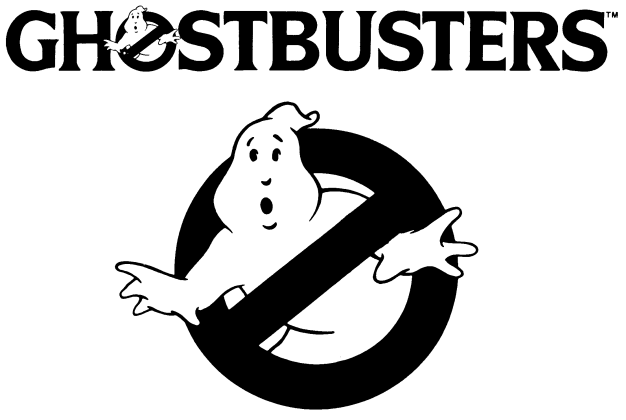
\includegraphics[width=1.0\textwidth]{ghostbusters-full.png}
\end{center}

\vspace{0.7cm}

\mysection{Introduction}

\myindent \href{https://en.wikipedia.org/wiki/Ghostbusters_(role-playing_game)}{Ghostbusters} est un jeu de rôles humoristique américain, conçu par \href{https://en.wikipedia.org/wiki/Sandy_Petersen}{Sandy Petersen}, \href{https://en.wikipedia.org/wiki/Lynn_Willis}{Lynn Willis} (les créateurs du jeu de rôles \href{https://en.wikipedia.org/wiki/Call_of_Cthulhu_(role-playing_game)}{Call of Cthulhu}), et \href{https://en.wikipedia.org/wiki/Greg_Stafford}{Greg Stafford} (le créateur de \href{https://en.wikipedia.org/wiki/RuneQuest}{Runequest} et de \href{https://en.wikipedia.org/wiki/Pendragon_(role-playing_game)}{Pendragon}), et publié en 1986 par \href{https://en.wikipedia.org/wiki/West_End_Games}{West End Games}.

\myindent Le système de jeu est très compact et très simple et vise des aventures amusantes dans l'univers des films. Il servira de fondation au \href{https://en.wikipedia.org/wiki/D6_System}{Système D6} dont \href{https://en.wikipedia.org/wiki/Star_Wars:_The_Roleplaying_Game}{Star Wars} est l'exemple le plus connu, et inspirera des dizaines de mini-jeux de rôles comme \href{https://rouboudou.itch.io/risus}{Risus}.

\myindent Ce document reprend les règles originales de 1986.

\vspace{0.2cm}

\begin{tabular}{p{3cm}p{5cm}}
Concepteur               & \copyright\ S. Petersen, L. Willis, G. Stafford \\
Version        &  Version originale 1986 \\
Traduction et adaptation & \textcopyleft\ O. Rey 2022 \\
Version                  & \myversion \\
Référence         & \myreference \\ 
\end{tabular}

\vspace{0.4cm}

%=================================================SECTION
\mysection{Création du personnage}

\mysubsection{Traits}

\myindent Les Ghostbusters possèdent quatre \textbf{Traits} :
\begin{myitemize}
\item Sa \textbf{Cervelle} (Brains),
\item Ses \textbf{Muscles} (Muscles),
\item Ses \textbf{Mouvements} (Moves),
\item Sa \textbf{Coolitude} (Cool).
\end{myitemize}

\myindent On assigne à chaque Trait une valeur numérique. Plus cette valeur est haute, meilleure est la performance du PJ qui l'utilise. Chaque joueur possède 12 points à répartir sur les 4 traits, sachant que la valeur d'un trait ne peut être ni inférieure à 1, ni supérieure à 5.

\myindent \textit{Note} : certains Ghostbusters ont plus de 5 points dans certains Traits, mais c'est le fruit de l'expérience (voir plus loin).

\myindent Lors d'une action dont l'issue n'est pas connue d'avance, le Ghostmaster assignera un \textbf{Facteur de Difficulté} (FD) à l'action. Le joueur devra lancer un nombre de \textbf{dés à 6 faces} correspondant au Trait associé, et son score devra être supérieur ou égal au FD pour que l'action réussisse. Un de ces dés doit être un \textbf{Dé Fantôme} (DF), un dé à 6 faces de couleur différente ayant un fantôme à la place du 6 (ou géré comme tel).

\mysubsection{Talents}

\myindent Les Ghostbusters ont un \textbf{Talent} par Trait. Quand le PJ tente une action pour laquelle il possède un Talent, le joueur lancera 3D de plus que son Trait.

\myindent Chaque joueur doit choisir un Talent par Trait dans les listes ci-dessous. Il est possible de choisir un Talent non listé si le MJ l'accepte (dans la plupart des scénarios de Ghosbusters RPG, les PNJ ont des Talents ne figurant pas dans ces listes).
}{
\begin{center}
\begin{tabular}{ccc}
&\textbf{Cervelle}&\\
Anthropologie & Déduction & Occultisme \\ 
Archéologie & Deviner & Parapsychologie \\
Astronomie & Électronique &  Physique \\ 
Bibliothèque scientifique & Faits sportifs & Psychanalyse \\ 
Biologie & Géologie & Réparation électrique \\
Botanique & Histoire & Réparation mécanique \\
Bureaucratie & Journalisme & Romans à l'eau de rose \\
Chimie & Linguistique & Zoologie \\
Coiffure à la mode & Mathématiques & \\
Comptabilité & Médecine & \\
\end{tabular}
\end{center}

\begin{center}
\begin{tabular}{cc>{\centering\arraybackslash}p{2.5cm}}
& \textbf{Muscles} &  \\
Bagarre & Escalader & Lutte \\
Casser des choses & Éventrer & Nager \\
Renverser à coups de pieds & Gloutonnerie & Sauter \\
Courir & Intimider & Soulever \\
\end{tabular}
\end{center}

\begin{center}
\begin{tabular}{ccc}
& \textbf{Mouvements} & \\
Attirer l'attention & Faire de la musique & Se déguiser \\
Attraper & Fouiner & Se pavaner \\
Breakdance & Furtivité & Séduire \\
Conduire un véhicule & Jeter & Tirer avec une arme \\
Écouter & Pickpocket & Tours de passe-passe \\
Équilibre & Ragots & Voir \\
Esquiver & Se cacher &  \\
\end{tabular}
\end{center}

\begin{center}
\begin{tabular}{>{\centering\arraybackslash}p{2.5cm}cc}
& \textbf{Coolitude} & \\
Bluffer & Élever des enfants & Jouer à la Bourse \\
Charmer & Emprunter & Marchander \\
Confusionner & Intimider & Orateur \\
Convaincre & Jouer au Poker & Raconter des bobards \\
\end{tabular}
\end{center}

\mysubsection{Bons Points}

\myindent Tous les Ghostbusters commencent le jeu avec 20 \textbf{Bons Points} (BP). Des BP seront gagnés quand ils auront fini les missions ou auront achevé leurs objectifs.

\myindent Quand les Ghostbusters vont mal, ils perdent des BP et prennent des amendes pour stationnement interdit, des appels injurieux de leurs créditeurs ou de longs séjours à l'hôpital.

\myindent Les Bons Points sont plus qu'une mesure de l'état de santé des Ghostbusters, ce sont des moyens pour eux d'influer sur l'histoire, de les voir tenter d'incroyables prouesses ou de les sortir de terribles ennuis.

\begin{center}
\begin{tabular}{cc}
\textbf{Action} & \textbf{Coût en BP}\\
Augmenter ses chances de succès\textsuperscript{1} & 1 BP = +1D au jet \\
Réduire le temps de séjour à l'hôpital & 1 BP = $-1$ semaine \\
Compenser une action très stupide & Un certain nombre de BP \\
Éviter de mourir & Un certain nombre de BP \\
\end{tabular}
\end{center}

{\small \textit{\textsuperscript{1} La décision de dépenser des Bons Points doit être faite avant le jet et ne peut pas modifier un jet déjà réalisé.}}

\mysubsection{Liens entre Bons Points et Traits}

\myindent Les Traits sont liés avec les BP de la manière suivante (avec accord du Ghostmaster) :

\begin{center}
\begin{tabular}{ccc}
\textbf{Contexte} & \textbf{Action} & \textbf{Impact en BP}\\
Expérience & Faire +1 sur un Trait & $-30$ BP \\
Moment critique\textsuperscript{2} & Faire $-1$ sur un Trait & +20 BP \\
\end{tabular}
\end{center}

{\small \textit{\textsuperscript{2} Par exemple, au lieu de mourir, un Ghostbuster n'ayant plus de BP peut en retrouver en perdant définitivement 1 point sur un de ses Traits.}}

\myindent Quand les BP sont utilisés par les joueurs pour sortir le Ghostbuster d'une mauvaise situation, ces derniers doivent décrire la situation. Si la description est amusante, le Ghostmaster pourra gratifier le Ghostbuster d'un bonus de +1 ou +2 BP.

\mysubsection{Expérience}

\myindent Le gain de BP après une mission est évalué comme suit :

\begin{center}\begin{tabular}{>{\centering\arraybackslash}p{3cm}>{\centering\arraybackslash}p{5cm}}
\textbf{Situation} & \textbf{Gain en BP}\\
Mission échouée ou fantôme non capturé & La moitié des BP perdus pendant la mission \\
Mission réussie & La totalité des BP récupérés, voire un léger bonus \\
Mission accomplie avec panache et fun & Tous les BP sont récupérés + la moitié des BP perdus pendant la mission \\
\end{tabular}
\end{center}


}
\end{frame}

%=======================================
%=======================================
%TODO Frame 2
\begin{frame}[b]

\deuxcolonnesbottom{%col1

%\begin{minipage}[c][0.95\textheight][c]{\linewidth}

\mysubsection{Objectif Personnel}

\myindent Le Ghostbuster poursuit un \textbf{Objectif Personnel}. L'atteindre lui accordera de nouveaux BP. La liste est donnée ci-dessous, sachant que le Ghostmaster peut valider un objectif n'étant pas dans la liste.

\myindent \textbf{Sexe} -- Le Ghostbuster est habitué à des relations sans lendemain. Si le Ghostbuster réussit à avoir un rendez-vous amoureux qui se passe bien durant une aventure : +1DF en BP.

\myindent Si le Fantôme est tiré, le Ghostbuster fait une grosse bêtise pendant le rendez-vous et ne gagne pas de BP (mais en gagnera un de plus au prochain jet réussi)


%\end{minipage}
}
{
%\begin{minipage}[c][0.95\textheight][c]{\linewidth}


%\end{minipage}
}
\end{frame}

